\batchmode
\documentclass[twoside]{book}

% Packages required by doxygen
\usepackage{fixltx2e}
\usepackage{calc}
\usepackage{doxygen}
\usepackage[export]{adjustbox} % also loads graphicx
\usepackage{graphicx}
\usepackage[utf8]{inputenc}
\usepackage{makeidx}
\usepackage{multicol}
\usepackage{multirow}
\PassOptionsToPackage{warn}{textcomp}
\usepackage{textcomp}
\usepackage[nointegrals]{wasysym}
\usepackage[table]{xcolor}

% Font selection
\usepackage[T1]{fontenc}
\usepackage[scaled=.90]{helvet}
\usepackage{courier}
\usepackage{amssymb}
\usepackage{sectsty}
\renewcommand{\familydefault}{\sfdefault}
\allsectionsfont{%
  \fontseries{bc}\selectfont%
  \color{darkgray}%
}
\renewcommand{\DoxyLabelFont}{%
  \fontseries{bc}\selectfont%
  \color{darkgray}%
}
\newcommand{\+}{\discretionary{\mbox{\scriptsize$\hookleftarrow$}}{}{}}

% Page & text layout
\usepackage{geometry}
\geometry{%
  a4paper,%
  top=2.5cm,%
  bottom=2.5cm,%
  left=2.5cm,%
  right=2.5cm%
}
\tolerance=750
\hfuzz=15pt
\hbadness=750
\setlength{\emergencystretch}{15pt}
\setlength{\parindent}{0cm}
\setlength{\parskip}{3ex plus 2ex minus 2ex}
\makeatletter
\renewcommand{\paragraph}{%
  \@startsection{paragraph}{4}{0ex}{-1.0ex}{1.0ex}{%
    \normalfont\normalsize\bfseries\SS@parafont%
  }%
}
\renewcommand{\subparagraph}{%
  \@startsection{subparagraph}{5}{0ex}{-1.0ex}{1.0ex}{%
    \normalfont\normalsize\bfseries\SS@subparafont%
  }%
}
\makeatother

% Headers & footers
\usepackage{fancyhdr}
\pagestyle{fancyplain}
\fancyhead[LE]{\fancyplain{}{\bfseries\thepage}}
\fancyhead[CE]{\fancyplain{}{}}
\fancyhead[RE]{\fancyplain{}{\bfseries\leftmark}}
\fancyhead[LO]{\fancyplain{}{\bfseries\rightmark}}
\fancyhead[CO]{\fancyplain{}{}}
\fancyhead[RO]{\fancyplain{}{\bfseries\thepage}}
\fancyfoot[LE]{\fancyplain{}{}}
\fancyfoot[CE]{\fancyplain{}{}}
\fancyfoot[RE]{\fancyplain{}{\bfseries\scriptsize Generated by Doxygen }}
\fancyfoot[LO]{\fancyplain{}{\bfseries\scriptsize Generated by Doxygen }}
\fancyfoot[CO]{\fancyplain{}{}}
\fancyfoot[RO]{\fancyplain{}{}}
\renewcommand{\footrulewidth}{0.4pt}
\renewcommand{\chaptermark}[1]{%
  \markboth{#1}{}%
}
\renewcommand{\sectionmark}[1]{%
  \markright{\thesection\ #1}%
}

% Indices & bibliography
\usepackage{natbib}
\usepackage[titles]{tocloft}
\setcounter{tocdepth}{3}
\setcounter{secnumdepth}{5}
\makeindex

% Hyperlinks (required, but should be loaded last)
\usepackage{ifpdf}
\ifpdf
  \usepackage[pdftex,pagebackref=true]{hyperref}
\else
  \usepackage[ps2pdf,pagebackref=true]{hyperref}
\fi
\hypersetup{%
  colorlinks=true,%
  linkcolor=blue,%
  citecolor=blue,%
  unicode%
}

% Custom commands
\newcommand{\clearemptydoublepage}{%
  \newpage{\pagestyle{empty}\cleardoublepage}%
}

\usepackage{caption}
\captionsetup{labelsep=space,justification=centering,font={bf},singlelinecheck=off,skip=4pt,position=top}

%===== C O N T E N T S =====

\begin{document}

% Titlepage & ToC
\hypersetup{pageanchor=false,
             bookmarksnumbered=true
            }
\pagenumbering{alph}
\pagenumbering{arabic}
\hypersetup{pageanchor=true}

%--- Begin generated contents ---
\chapter{Demo problem\+: Large-\/displacement post-\/buckling of a pressure-\/loaded thin-\/walled elastic ring -\/-\/ displacement-\/control techniques}
\label{index}\hypertarget{index}{}\hypertarget{index_q}{}\section{A few quick questions...}\label{index_q}
Since {\ttfamily oomph-\/lib} is developed as open-\/source software, any evidence that the code is being downloaded and used is very helpful for us as it helps to justify our continued work on this project.

We would therefore be extremely grateful if you could provide the information requested in the form below. Pressing the \char`\"{}submit\char`\"{} button will get you to the actual download page.

{\bfseries Note\+:} 
\begin{DoxyItemize}
\item All information will be treated as confidential. 
\item If you provide your email address and check the appropriate box we will add you to our mailing list to inform you of upgrades and bug fixes to the code. Rest assured that the mailing list is {\bfseries very low volume} -- we have better things to do than to bombard you with email. 
\item If you still feel reluctant to provide any of the information requested, feel free to enter some dummy input. The form will check that {\bfseries some} information has been entered but entering your name as \char`\"{}\+Joe Cool\char`\"{} is perfectly acceptable -- this is to discourage people from not providing the information simply because they are too lazy to type... 
\end{DoxyItemize}



 







 

 \hypertarget{index_pdf}{}\section{P\+D\+F file}\label{index_pdf}
A \href{../latex/refman.pdf}{\tt pdf version} of this document is available. \end{document}

\chapter{Namespace Index}
\section{Namespace List}
Here is a list of all namespaces with brief descriptions\+:\begin{DoxyCompactList}
\item\contentsline{section}{\hyperlink{namespaceGlobal__Physical__Variables}{Global\+\_\+\+Physical\+\_\+\+Variables} \\*Global variables that represent physical properties }{\pageref{namespaceGlobal__Physical__Variables}}{}
\item\contentsline{section}{\hyperlink{namespaceoomph}{oomph} }{\pageref{namespaceoomph}}{}
\item\contentsline{section}{\hyperlink{namespacePhysical__Variables}{Physical\+\_\+\+Variables} \\*Namespace for the solution of 2D linear shell equation }{\pageref{namespacePhysical__Variables}}{}
\end{DoxyCompactList}

\chapter{Hierarchical Index}
\section{Class Hierarchy}
This inheritance list is sorted roughly, but not completely, alphabetically\+:\begin{DoxyCompactList}
\item Problem\begin{DoxyCompactList}
\item \contentsline{section}{Unstructured\+Solid\+Problem$<$ E\+L\+E\+M\+E\+NT $>$}{\pageref{classUnstructuredSolidProblem}}{}
\end{DoxyCompactList}
\end{DoxyCompactList}

\chapter{Class Index}
\section{Class List}
Here are the classes, structs, unions and interfaces with brief descriptions\+:\begin{DoxyCompactList}
\item\contentsline{section}{\hyperlink{classPMLProblem}{P\+M\+L\+Problem$<$ E\+L\+E\+M\+E\+N\+T $>$} }{\pageref{classPMLProblem}}{}
\item\contentsline{section}{\hyperlink{classGlobalParameters_1_1TestPMLMapping}{Global\+Parameters\+::\+Test\+P\+M\+L\+Mapping} }{\pageref{classGlobalParameters_1_1TestPMLMapping}}{}
\end{DoxyCompactList}

\chapter{File Index}
\section{File List}
Here is a list of all files with brief descriptions\+:\begin{DoxyCompactList}
\item\contentsline{section}{\hyperlink{jeffery__orbit_8cc}{jeffery\+\_\+orbit.\+cc} }{\pageref{jeffery__orbit_8cc}}{}
\item\contentsline{section}{\hyperlink{jeffery__orbit_8txt__doxygenified_8h}{jeffery\+\_\+orbit.\+txt\+\_\+doxygenified.\+h} }{\pageref{jeffery__orbit_8txt__doxygenified_8h}}{}
\item\contentsline{section}{\hyperlink{my__taylor__hood__elements_8h}{my\+\_\+taylor\+\_\+hood\+\_\+elements.\+h} }{\pageref{my__taylor__hood__elements_8h}}{}
\end{DoxyCompactList}

\chapter{Namespace Documentation}
\hypertarget{namespaceGlobal__Physical__Variables}{}\section{Global\+\_\+\+Physical\+\_\+\+Variables Namespace Reference}
\label{namespaceGlobal__Physical__Variables}\index{Global\+\_\+\+Physical\+\_\+\+Variables@{Global\+\_\+\+Physical\+\_\+\+Variables}}


Namespace for physical parameters.  


\subsection*{Functions}
\begin{DoxyCompactItemize}
\item 
Vector$<$ double $>$ \hyperlink{namespaceGlobal__Physical__Variables_afae321364975eb56688ad13abc8ed6b7}{Gravity} (2)
\begin{DoxyCompactList}\small\item\em Gravity vector. \end{DoxyCompactList}\item 
void \hyperlink{namespaceGlobal__Physical__Variables_a87da705b8a46bed337cf5dbdd788b87b}{body\+\_\+force} (const double \&time, const Vector$<$ double $>$ \&x, Vector$<$ double $>$ \&result)
\begin{DoxyCompactList}\small\item\em Functional body force. \end{DoxyCompactList}\item 
void \hyperlink{namespaceGlobal__Physical__Variables_a9780d615ae07c4e00a436ab2973b54e6}{zero\+\_\+body\+\_\+force} (const double \&time, const Vector$<$ double $>$ \&x, Vector$<$ double $>$ \&result)
\begin{DoxyCompactList}\small\item\em Zero functional body force. \end{DoxyCompactList}\end{DoxyCompactItemize}
\subsection*{Variables}
\begin{DoxyCompactItemize}
\item 
double \hyperlink{namespaceGlobal__Physical__Variables_ab814e627d2eb5bc50318879d19ab16b9}{Re} =100
\begin{DoxyCompactList}\small\item\em Reynolds number. \end{DoxyCompactList}\item 
double \hyperlink{namespaceGlobal__Physical__Variables_ab1a845a672b4d74b304639a976dc65c6}{Re\+\_\+inv\+Fr} =100
\begin{DoxyCompactList}\small\item\em Reynolds/\+Froude number. \end{DoxyCompactList}\end{DoxyCompactItemize}


\subsection{Detailed Description}
Namespace for physical parameters. 

\subsection{Function Documentation}
\mbox{\Hypertarget{namespaceGlobal__Physical__Variables_a87da705b8a46bed337cf5dbdd788b87b}\label{namespaceGlobal__Physical__Variables_a87da705b8a46bed337cf5dbdd788b87b}} 
\index{Global\+\_\+\+Physical\+\_\+\+Variables@{Global\+\_\+\+Physical\+\_\+\+Variables}!body\+\_\+force@{body\+\_\+force}}
\index{body\+\_\+force@{body\+\_\+force}!Global\+\_\+\+Physical\+\_\+\+Variables@{Global\+\_\+\+Physical\+\_\+\+Variables}}
\subsubsection{\texorpdfstring{body\+\_\+force()}{body\_force()}}
{\footnotesize\ttfamily void Global\+\_\+\+Physical\+\_\+\+Variables\+::body\+\_\+force (\begin{DoxyParamCaption}\item[{const double \&}]{time,  }\item[{const Vector$<$ double $>$ \&}]{x,  }\item[{Vector$<$ double $>$ \&}]{result }\end{DoxyParamCaption})}



Functional body force. 



Definition at line 62 of file circular\+\_\+driven\+\_\+cavity.\+cc.



References Re\+\_\+inv\+Fr.



Referenced by main().

\mbox{\Hypertarget{namespaceGlobal__Physical__Variables_afae321364975eb56688ad13abc8ed6b7}\label{namespaceGlobal__Physical__Variables_afae321364975eb56688ad13abc8ed6b7}} 
\index{Global\+\_\+\+Physical\+\_\+\+Variables@{Global\+\_\+\+Physical\+\_\+\+Variables}!Gravity@{Gravity}}
\index{Gravity@{Gravity}!Global\+\_\+\+Physical\+\_\+\+Variables@{Global\+\_\+\+Physical\+\_\+\+Variables}}
\subsubsection{\texorpdfstring{Gravity()}{Gravity()}}
{\footnotesize\ttfamily Vector$<$double$>$ Global\+\_\+\+Physical\+\_\+\+Variables\+::\+Gravity (\begin{DoxyParamCaption}\item[{2}]{ }\end{DoxyParamCaption})}



Gravity vector. 



Referenced by main(), and Quarter\+Circle\+Driven\+Cavity\+Problem$<$ E\+L\+E\+M\+E\+N\+T $>$\+::\+Quarter\+Circle\+Driven\+Cavity\+Problem().

\mbox{\Hypertarget{namespaceGlobal__Physical__Variables_a9780d615ae07c4e00a436ab2973b54e6}\label{namespaceGlobal__Physical__Variables_a9780d615ae07c4e00a436ab2973b54e6}} 
\index{Global\+\_\+\+Physical\+\_\+\+Variables@{Global\+\_\+\+Physical\+\_\+\+Variables}!zero\+\_\+body\+\_\+force@{zero\+\_\+body\+\_\+force}}
\index{zero\+\_\+body\+\_\+force@{zero\+\_\+body\+\_\+force}!Global\+\_\+\+Physical\+\_\+\+Variables@{Global\+\_\+\+Physical\+\_\+\+Variables}}
\subsubsection{\texorpdfstring{zero\+\_\+body\+\_\+force()}{zero\_body\_force()}}
{\footnotesize\ttfamily void Global\+\_\+\+Physical\+\_\+\+Variables\+::zero\+\_\+body\+\_\+force (\begin{DoxyParamCaption}\item[{const double \&}]{time,  }\item[{const Vector$<$ double $>$ \&}]{x,  }\item[{Vector$<$ double $>$ \&}]{result }\end{DoxyParamCaption})}



Zero functional body force. 



Definition at line 70 of file circular\+\_\+driven\+\_\+cavity.\+cc.



Referenced by main().



\subsection{Variable Documentation}
\mbox{\Hypertarget{namespaceGlobal__Physical__Variables_ab814e627d2eb5bc50318879d19ab16b9}\label{namespaceGlobal__Physical__Variables_ab814e627d2eb5bc50318879d19ab16b9}} 
\index{Global\+\_\+\+Physical\+\_\+\+Variables@{Global\+\_\+\+Physical\+\_\+\+Variables}!Re@{Re}}
\index{Re@{Re}!Global\+\_\+\+Physical\+\_\+\+Variables@{Global\+\_\+\+Physical\+\_\+\+Variables}}
\subsubsection{\texorpdfstring{Re}{Re}}
{\footnotesize\ttfamily double Global\+\_\+\+Physical\+\_\+\+Variables\+::\+Re =100}



Reynolds number. 



Definition at line 53 of file circular\+\_\+driven\+\_\+cavity.\+cc.



Referenced by Quarter\+Circle\+Driven\+Cavity\+Problem$<$ E\+L\+E\+M\+E\+N\+T $>$\+::\+Quarter\+Circle\+Driven\+Cavity\+Problem().

\mbox{\Hypertarget{namespaceGlobal__Physical__Variables_ab1a845a672b4d74b304639a976dc65c6}\label{namespaceGlobal__Physical__Variables_ab1a845a672b4d74b304639a976dc65c6}} 
\index{Global\+\_\+\+Physical\+\_\+\+Variables@{Global\+\_\+\+Physical\+\_\+\+Variables}!Re\+\_\+inv\+Fr@{Re\+\_\+inv\+Fr}}
\index{Re\+\_\+inv\+Fr@{Re\+\_\+inv\+Fr}!Global\+\_\+\+Physical\+\_\+\+Variables@{Global\+\_\+\+Physical\+\_\+\+Variables}}
\subsubsection{\texorpdfstring{Re\+\_\+inv\+Fr}{Re\_invFr}}
{\footnotesize\ttfamily double Global\+\_\+\+Physical\+\_\+\+Variables\+::\+Re\+\_\+inv\+Fr =100}



Reynolds/\+Froude number. 



Definition at line 56 of file circular\+\_\+driven\+\_\+cavity.\+cc.



Referenced by body\+\_\+force(), and Quarter\+Circle\+Driven\+Cavity\+Problem$<$ E\+L\+E\+M\+E\+N\+T $>$\+::\+Quarter\+Circle\+Driven\+Cavity\+Problem().


\chapter{Class Documentation}
\hypertarget{classElasticRingProblem}{}\section{Elastic\+Ring\+Problem$<$ E\+L\+E\+M\+E\+NT $>$ Class Template Reference}
\label{classElasticRingProblem}\index{Elastic\+Ring\+Problem$<$ E\+L\+E\+M\+E\+N\+T $>$@{Elastic\+Ring\+Problem$<$ E\+L\+E\+M\+E\+N\+T $>$}}


Ring problem.  


Inheritance diagram for Elastic\+Ring\+Problem$<$ E\+L\+E\+M\+E\+NT $>$\+:\begin{figure}[H]
\begin{center}
\leavevmode
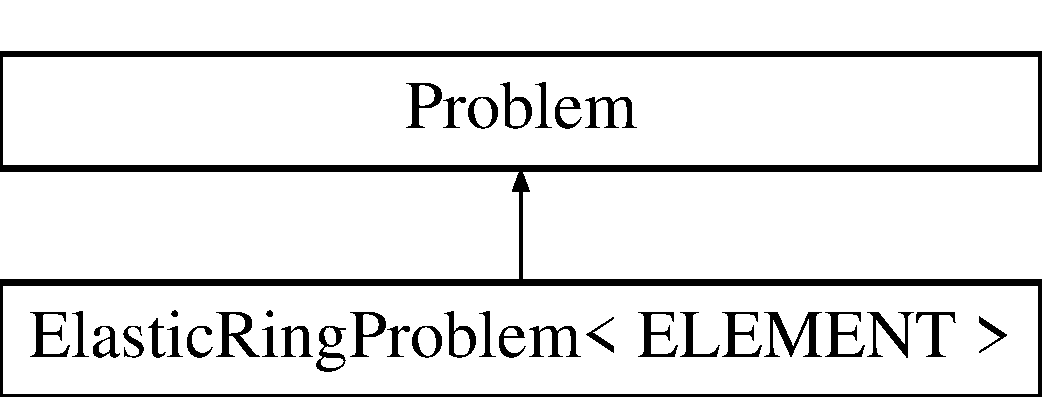
\includegraphics[height=2.000000cm]{classElasticRingProblem}
\end{center}
\end{figure}
\subsection*{Public Member Functions}
\begin{DoxyCompactItemize}
\item 
\hyperlink{classElasticRingProblem_a46779ff320754561750e22216f7605e3}{Elastic\+Ring\+Problem} (const unsigned \&n\+\_\+element, bool \&displ\+\_\+control, bool \&load\+\_\+data\+\_\+already\+\_\+exists)
\begin{DoxyCompactList}\small\item\em Constructor for elastic ring problem. \end{DoxyCompactList}\item 
One\+D\+Lagrangian\+Mesh$<$ E\+L\+E\+M\+E\+NT $>$ $\ast$ \hyperlink{classElasticRingProblem_a7e956ca937741ce71cf400eb492825b3}{mesh\+\_\+pt} ()
\begin{DoxyCompactList}\small\item\em Access function for the specific mesh. \end{DoxyCompactList}\item 
void \hyperlink{classElasticRingProblem_a58c2889fd4db8c17f4a4d964a5a7a90d}{actions\+\_\+after\+\_\+newton\+\_\+solve} ()
\begin{DoxyCompactList}\small\item\em Update function is empty. \end{DoxyCompactList}\item 
void \hyperlink{classElasticRingProblem_a6d084ac04c73a116f5ece449935a31d3}{actions\+\_\+before\+\_\+newton\+\_\+solve} ()
\begin{DoxyCompactList}\small\item\em Update function is empty. \end{DoxyCompactList}\item 
void \hyperlink{classElasticRingProblem_ab644c5fd57310f2d4c858f64d8c5a223}{doc\+\_\+solution} (Doc\+Info \&doc\+\_\+info, ofstream \&trace\+\_\+file)
\begin{DoxyCompactList}\small\item\em Doc solution. \end{DoxyCompactList}\item 
void \hyperlink{classElasticRingProblem_afed9c0948c535c315c3e22e92e3266d3}{parameter\+\_\+study} (Doc\+Info \&doc\+\_\+info)
\begin{DoxyCompactList}\small\item\em Perform the parameter study. \end{DoxyCompactList}\end{DoxyCompactItemize}
\subsection*{Private Attributes}
\begin{DoxyCompactItemize}
\item 
bool \hyperlink{classElasticRingProblem_a919d11c9d2167d909c4d4563e9ca83b6}{Displ\+\_\+control}
\begin{DoxyCompactList}\small\item\em Use displacement control? \end{DoxyCompactList}\item 
Geom\+Object $\ast$ \hyperlink{classElasticRingProblem_a08e4afcece28aee2d1ee2e6c54394be8}{Undef\+\_\+geom\+\_\+pt}
\begin{DoxyCompactList}\small\item\em Pointer to geometric object that represents the undeformed shape. \end{DoxyCompactList}\item 
unsigned \hyperlink{classElasticRingProblem_aa57e3dd4e9a5187ef7394b019e68b1ca}{Nbeam\+\_\+element}
\begin{DoxyCompactList}\small\item\em Number of elements in the beam mesh. \end{DoxyCompactList}\end{DoxyCompactItemize}


\subsection{Detailed Description}
\subsubsection*{template$<$class E\+L\+E\+M\+E\+NT$>$\newline
class Elastic\+Ring\+Problem$<$ E\+L\+E\+M\+E\+N\+T $>$}

Ring problem. 

Definition at line 101 of file steady\+\_\+ring.\+cc.



\subsection{Constructor \& Destructor Documentation}
\mbox{\Hypertarget{classElasticRingProblem_a46779ff320754561750e22216f7605e3}\label{classElasticRingProblem_a46779ff320754561750e22216f7605e3}} 
\index{Elastic\+Ring\+Problem@{Elastic\+Ring\+Problem}!Elastic\+Ring\+Problem@{Elastic\+Ring\+Problem}}
\index{Elastic\+Ring\+Problem@{Elastic\+Ring\+Problem}!Elastic\+Ring\+Problem@{Elastic\+Ring\+Problem}}
\subsubsection{\texorpdfstring{Elastic\+Ring\+Problem()}{ElasticRingProblem()}}
{\footnotesize\ttfamily template$<$class E\+L\+E\+M\+E\+NT $>$ \\
\hyperlink{classElasticRingProblem}{Elastic\+Ring\+Problem}$<$ E\+L\+E\+M\+E\+NT $>$\+::\hyperlink{classElasticRingProblem}{Elastic\+Ring\+Problem} (\begin{DoxyParamCaption}\item[{const unsigned \&}]{n\+\_\+element,  }\item[{bool \&}]{displ\+\_\+control,  }\item[{bool \&}]{load\+\_\+data\+\_\+already\+\_\+exists }\end{DoxyParamCaption})}



Constructor for elastic ring problem. 

Constructor\+: Number of elements and flags for displ control and displacement control with existing data respectively. 

Definition at line 154 of file steady\+\_\+ring.\+cc.



References Global\+\_\+\+Physical\+\_\+\+Variables\+::H, Global\+\_\+\+Physical\+\_\+\+Variables\+::\+Pext\+\_\+data\+\_\+pt, Global\+\_\+\+Physical\+\_\+\+Variables\+::press\+\_\+load(), and Global\+\_\+\+Physical\+\_\+\+Variables\+::\+Xprescr.



\subsection{Member Function Documentation}
\mbox{\Hypertarget{classElasticRingProblem_a58c2889fd4db8c17f4a4d964a5a7a90d}\label{classElasticRingProblem_a58c2889fd4db8c17f4a4d964a5a7a90d}} 
\index{Elastic\+Ring\+Problem@{Elastic\+Ring\+Problem}!actions\+\_\+after\+\_\+newton\+\_\+solve@{actions\+\_\+after\+\_\+newton\+\_\+solve}}
\index{actions\+\_\+after\+\_\+newton\+\_\+solve@{actions\+\_\+after\+\_\+newton\+\_\+solve}!Elastic\+Ring\+Problem@{Elastic\+Ring\+Problem}}
\subsubsection{\texorpdfstring{actions\+\_\+after\+\_\+newton\+\_\+solve()}{actions\_after\_newton\_solve()}}
{\footnotesize\ttfamily template$<$class E\+L\+E\+M\+E\+NT$>$ \\
void \hyperlink{classElasticRingProblem}{Elastic\+Ring\+Problem}$<$ E\+L\+E\+M\+E\+NT $>$\+::actions\+\_\+after\+\_\+newton\+\_\+solve (\begin{DoxyParamCaption}{ }\end{DoxyParamCaption})\hspace{0.3cm}{\ttfamily [inline]}}



Update function is empty. 



Definition at line 119 of file steady\+\_\+ring.\+cc.

\mbox{\Hypertarget{classElasticRingProblem_a6d084ac04c73a116f5ece449935a31d3}\label{classElasticRingProblem_a6d084ac04c73a116f5ece449935a31d3}} 
\index{Elastic\+Ring\+Problem@{Elastic\+Ring\+Problem}!actions\+\_\+before\+\_\+newton\+\_\+solve@{actions\+\_\+before\+\_\+newton\+\_\+solve}}
\index{actions\+\_\+before\+\_\+newton\+\_\+solve@{actions\+\_\+before\+\_\+newton\+\_\+solve}!Elastic\+Ring\+Problem@{Elastic\+Ring\+Problem}}
\subsubsection{\texorpdfstring{actions\+\_\+before\+\_\+newton\+\_\+solve()}{actions\_before\_newton\_solve()}}
{\footnotesize\ttfamily template$<$class E\+L\+E\+M\+E\+NT$>$ \\
void \hyperlink{classElasticRingProblem}{Elastic\+Ring\+Problem}$<$ E\+L\+E\+M\+E\+NT $>$\+::actions\+\_\+before\+\_\+newton\+\_\+solve (\begin{DoxyParamCaption}{ }\end{DoxyParamCaption})\hspace{0.3cm}{\ttfamily [inline]}}



Update function is empty. 



Definition at line 122 of file steady\+\_\+ring.\+cc.

\mbox{\Hypertarget{classElasticRingProblem_ab644c5fd57310f2d4c858f64d8c5a223}\label{classElasticRingProblem_ab644c5fd57310f2d4c858f64d8c5a223}} 
\index{Elastic\+Ring\+Problem@{Elastic\+Ring\+Problem}!doc\+\_\+solution@{doc\+\_\+solution}}
\index{doc\+\_\+solution@{doc\+\_\+solution}!Elastic\+Ring\+Problem@{Elastic\+Ring\+Problem}}
\subsubsection{\texorpdfstring{doc\+\_\+solution()}{doc\_solution()}}
{\footnotesize\ttfamily template$<$class E\+L\+E\+M\+E\+NT $>$ \\
void \hyperlink{classElasticRingProblem}{Elastic\+Ring\+Problem}$<$ E\+L\+E\+M\+E\+NT $>$\+::doc\+\_\+solution (\begin{DoxyParamCaption}\item[{Doc\+Info \&}]{doc\+\_\+info,  }\item[{ofstream \&}]{trace\+\_\+file }\end{DoxyParamCaption})}



Doc solution. 

Document solution. 

Definition at line 298 of file steady\+\_\+ring.\+cc.



References Global\+\_\+\+Physical\+\_\+\+Variables\+::H, and Global\+\_\+\+Physical\+\_\+\+Variables\+::\+Pext\+\_\+data\+\_\+pt.

\mbox{\Hypertarget{classElasticRingProblem_a7e956ca937741ce71cf400eb492825b3}\label{classElasticRingProblem_a7e956ca937741ce71cf400eb492825b3}} 
\index{Elastic\+Ring\+Problem@{Elastic\+Ring\+Problem}!mesh\+\_\+pt@{mesh\+\_\+pt}}
\index{mesh\+\_\+pt@{mesh\+\_\+pt}!Elastic\+Ring\+Problem@{Elastic\+Ring\+Problem}}
\subsubsection{\texorpdfstring{mesh\+\_\+pt()}{mesh\_pt()}}
{\footnotesize\ttfamily template$<$class E\+L\+E\+M\+E\+NT$>$ \\
One\+D\+Lagrangian\+Mesh$<$E\+L\+E\+M\+E\+NT$>$$\ast$ \hyperlink{classElasticRingProblem}{Elastic\+Ring\+Problem}$<$ E\+L\+E\+M\+E\+NT $>$\+::mesh\+\_\+pt (\begin{DoxyParamCaption}{ }\end{DoxyParamCaption})\hspace{0.3cm}{\ttfamily [inline]}}



Access function for the specific mesh. 



Definition at line 113 of file steady\+\_\+ring.\+cc.

\mbox{\Hypertarget{classElasticRingProblem_afed9c0948c535c315c3e22e92e3266d3}\label{classElasticRingProblem_afed9c0948c535c315c3e22e92e3266d3}} 
\index{Elastic\+Ring\+Problem@{Elastic\+Ring\+Problem}!parameter\+\_\+study@{parameter\+\_\+study}}
\index{parameter\+\_\+study@{parameter\+\_\+study}!Elastic\+Ring\+Problem@{Elastic\+Ring\+Problem}}
\subsubsection{\texorpdfstring{parameter\+\_\+study()}{parameter\_study()}}
{\footnotesize\ttfamily template$<$class E\+L\+E\+M\+E\+NT $>$ \\
void \hyperlink{classElasticRingProblem}{Elastic\+Ring\+Problem}$<$ E\+L\+E\+M\+E\+NT $>$\+::parameter\+\_\+study (\begin{DoxyParamCaption}\item[{Doc\+Info \&}]{doc\+\_\+info }\end{DoxyParamCaption})}



Perform the parameter study. 

Solver loop to perform parameter study. Perturbation pressure 

Definition at line 341 of file steady\+\_\+ring.\+cc.



References Global\+\_\+\+Physical\+\_\+\+Variables\+::external\+\_\+pressure(), Global\+\_\+\+Physical\+\_\+\+Variables\+::H, Global\+\_\+\+Physical\+\_\+\+Variables\+::\+Pcos, Global\+\_\+\+Physical\+\_\+\+Variables\+::\+Pext\+\_\+data\+\_\+pt, and Global\+\_\+\+Physical\+\_\+\+Variables\+::\+Xprescr.



Referenced by main().



\subsection{Member Data Documentation}
\mbox{\Hypertarget{classElasticRingProblem_a919d11c9d2167d909c4d4563e9ca83b6}\label{classElasticRingProblem_a919d11c9d2167d909c4d4563e9ca83b6}} 
\index{Elastic\+Ring\+Problem@{Elastic\+Ring\+Problem}!Displ\+\_\+control@{Displ\+\_\+control}}
\index{Displ\+\_\+control@{Displ\+\_\+control}!Elastic\+Ring\+Problem@{Elastic\+Ring\+Problem}}
\subsubsection{\texorpdfstring{Displ\+\_\+control}{Displ\_control}}
{\footnotesize\ttfamily template$<$class E\+L\+E\+M\+E\+NT$>$ \\
bool \hyperlink{classElasticRingProblem}{Elastic\+Ring\+Problem}$<$ E\+L\+E\+M\+E\+NT $>$\+::Displ\+\_\+control\hspace{0.3cm}{\ttfamily [private]}}



Use displacement control? 



Definition at line 133 of file steady\+\_\+ring.\+cc.

\mbox{\Hypertarget{classElasticRingProblem_aa57e3dd4e9a5187ef7394b019e68b1ca}\label{classElasticRingProblem_aa57e3dd4e9a5187ef7394b019e68b1ca}} 
\index{Elastic\+Ring\+Problem@{Elastic\+Ring\+Problem}!Nbeam\+\_\+element@{Nbeam\+\_\+element}}
\index{Nbeam\+\_\+element@{Nbeam\+\_\+element}!Elastic\+Ring\+Problem@{Elastic\+Ring\+Problem}}
\subsubsection{\texorpdfstring{Nbeam\+\_\+element}{Nbeam\_element}}
{\footnotesize\ttfamily template$<$class E\+L\+E\+M\+E\+NT$>$ \\
unsigned \hyperlink{classElasticRingProblem}{Elastic\+Ring\+Problem}$<$ E\+L\+E\+M\+E\+NT $>$\+::Nbeam\+\_\+element\hspace{0.3cm}{\ttfamily [private]}}



Number of elements in the beam mesh. 



Definition at line 139 of file steady\+\_\+ring.\+cc.

\mbox{\Hypertarget{classElasticRingProblem_a08e4afcece28aee2d1ee2e6c54394be8}\label{classElasticRingProblem_a08e4afcece28aee2d1ee2e6c54394be8}} 
\index{Elastic\+Ring\+Problem@{Elastic\+Ring\+Problem}!Undef\+\_\+geom\+\_\+pt@{Undef\+\_\+geom\+\_\+pt}}
\index{Undef\+\_\+geom\+\_\+pt@{Undef\+\_\+geom\+\_\+pt}!Elastic\+Ring\+Problem@{Elastic\+Ring\+Problem}}
\subsubsection{\texorpdfstring{Undef\+\_\+geom\+\_\+pt}{Undef\_geom\_pt}}
{\footnotesize\ttfamily template$<$class E\+L\+E\+M\+E\+NT$>$ \\
Geom\+Object$\ast$ \hyperlink{classElasticRingProblem}{Elastic\+Ring\+Problem}$<$ E\+L\+E\+M\+E\+NT $>$\+::Undef\+\_\+geom\+\_\+pt\hspace{0.3cm}{\ttfamily [private]}}



Pointer to geometric object that represents the undeformed shape. 



Definition at line 136 of file steady\+\_\+ring.\+cc.



The documentation for this class was generated from the following file\+:\begin{DoxyCompactItemize}
\item 
\hyperlink{steady__ring_8cc}{steady\+\_\+ring.\+cc}\end{DoxyCompactItemize}

\chapter{File Documentation}
\hypertarget{steady__ring_8cc}{}\section{steady\+\_\+ring.\+cc File Reference}
\label{steady__ring_8cc}\index{steady\+\_\+ring.\+cc@{steady\+\_\+ring.\+cc}}
\subsection*{Classes}
\begin{DoxyCompactItemize}
\item 
class \hyperlink{classElasticRingProblem}{Elastic\+Ring\+Problem$<$ E\+L\+E\+M\+E\+N\+T $>$}
\begin{DoxyCompactList}\small\item\em Ring problem. \end{DoxyCompactList}\end{DoxyCompactItemize}
\subsection*{Namespaces}
\begin{DoxyCompactItemize}
\item 
 \hyperlink{namespaceGlobal__Physical__Variables}{Global\+\_\+\+Physical\+\_\+\+Variables}
\begin{DoxyCompactList}\small\item\em Namespace for physical parameters. \end{DoxyCompactList}\end{DoxyCompactItemize}
\subsection*{Functions}
\begin{DoxyCompactItemize}
\item 
void \hyperlink{namespaceGlobal__Physical__Variables_a86fd8f502cb8c4c7939ffae742f023eb}{Global\+\_\+\+Physical\+\_\+\+Variables\+::press\+\_\+load} (const Vector$<$ double $>$ \&xi, const Vector$<$ double $>$ \&x, const Vector$<$ double $>$ \&N, Vector$<$ double $>$ \&load)
\begin{DoxyCompactList}\small\item\em Load function\+: Constant external pressure with cos variation to induce buckling in n=2 mode. \end{DoxyCompactList}\item 
double \& \hyperlink{namespaceGlobal__Physical__Variables_a8c25ac6a672ea50d1b709292d1f4837b}{Global\+\_\+\+Physical\+\_\+\+Variables\+::external\+\_\+pressure} ()
\begin{DoxyCompactList}\small\item\em Return a reference to the external pressure load on the elastic ring. A reference is obtained by de-\/referencing the pointer to the data value that contains the external load. \end{DoxyCompactList}\item 
int \hyperlink{steady__ring_8cc_ae66f6b31b5ad750f1fe042a706a4e3d4}{main} ()
\begin{DoxyCompactList}\small\item\em Driver for ring test problem. \end{DoxyCompactList}\end{DoxyCompactItemize}
\subsection*{Variables}
\begin{DoxyCompactItemize}
\item 
double \hyperlink{namespaceGlobal__Physical__Variables_af6e07423e22c0991084d9a2f43727805}{Global\+\_\+\+Physical\+\_\+\+Variables\+::H} =0.\+05
\begin{DoxyCompactList}\small\item\em Nondim thickness. \end{DoxyCompactList}\item 
double \hyperlink{namespaceGlobal__Physical__Variables_a1c774c9cb221df909201e81e84b15f40}{Global\+\_\+\+Physical\+\_\+\+Variables\+::\+Xprescr} = 1.\+0
\begin{DoxyCompactList}\small\item\em Prescribed position (only used for displacement control) \end{DoxyCompactList}\item 
double \hyperlink{namespaceGlobal__Physical__Variables_ab55734aaa66260cd9d4bf68a4ecafdd5}{Global\+\_\+\+Physical\+\_\+\+Variables\+::\+Pcos} =0.\+0
\begin{DoxyCompactList}\small\item\em Perturbation pressure. \end{DoxyCompactList}\item 
Data $\ast$ \hyperlink{namespaceGlobal__Physical__Variables_a9d598320fb3d7ecf94101088e8f376d2}{Global\+\_\+\+Physical\+\_\+\+Variables\+::\+Pext\+\_\+data\+\_\+pt}
\begin{DoxyCompactList}\small\item\em Pointer to pressure load (stored in Data so it can become an unknown in the problem when displacement control is used. \end{DoxyCompactList}\end{DoxyCompactItemize}


\subsection{Function Documentation}
\mbox{\Hypertarget{steady__ring_8cc_ae66f6b31b5ad750f1fe042a706a4e3d4}\label{steady__ring_8cc_ae66f6b31b5ad750f1fe042a706a4e3d4}} 
\index{steady\+\_\+ring.\+cc@{steady\+\_\+ring.\+cc}!main@{main}}
\index{main@{main}!steady\+\_\+ring.\+cc@{steady\+\_\+ring.\+cc}}
\subsubsection{\texorpdfstring{main()}{main()}}
{\footnotesize\ttfamily int main (\begin{DoxyParamCaption}{ }\end{DoxyParamCaption})}



Driver for ring test problem. 



Definition at line 460 of file steady\+\_\+ring.\+cc.



References Elastic\+Ring\+Problem$<$ E\+L\+E\+M\+E\+N\+T $>$\+::parameter\+\_\+study().


\hypertarget{steady__ring_8txt__doxygenified_8h}{}\section{steady\+\_\+ring.\+txt\+\_\+doxygenified.\+h File Reference}
\label{steady__ring_8txt__doxygenified_8h}\index{steady\+\_\+ring.\+txt\+\_\+doxygenified.\+h@{steady\+\_\+ring.\+txt\+\_\+doxygenified.\+h}}

%--- End generated contents ---

% Index
\backmatter
\newpage
\phantomsection
\clearemptydoublepage
\addcontentsline{toc}{chapter}{Index}
\printindex

